\documentclass[a4paper,12pt]{article}
\usepackage[spanish]{babel}
\usepackage[utf8]{inputenc}
\usepackage{booktabs}
\usepackage{dirtytalk}
\usepackage{graphicx}
\usepackage{dirtytalk}
\usepackage[T1]{fontenc}
\usepackage[document]{ragged2e}

\begin{document}

\title{\Large Instituto Politécnico Nacional\\Escuela Superior de Cómputo\\Sistemas Operativos\\ Mapa mental Historia Unix y Linux \\Alumno: Meza Zamora Abraham Manuel\\Profesor: Ephra\'in Herrera Salgado}
\date{}
\maketitle

\section{Mapa mental} 
\begin{figure}[h]
\center
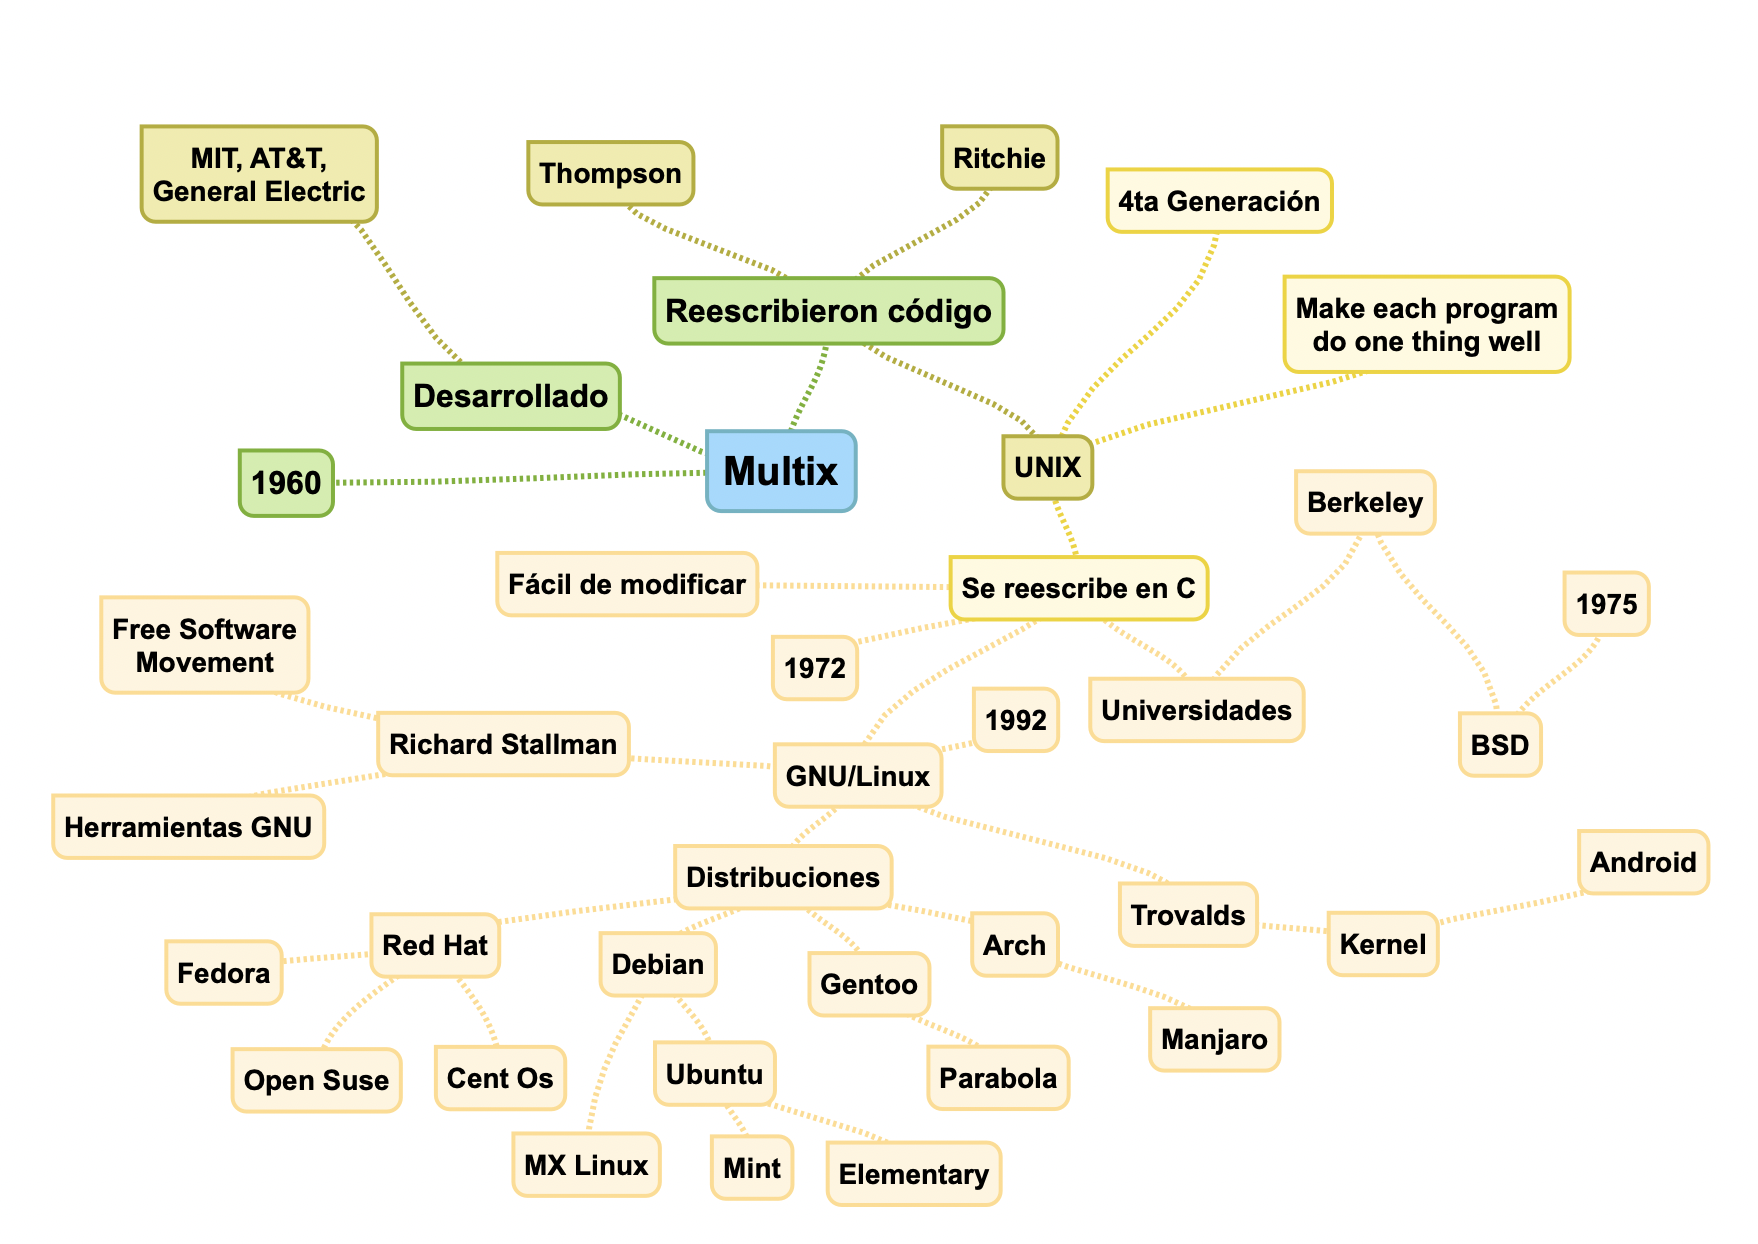
\includegraphics[scale=.35]{uno}
\caption{Mapa Generaciones de computadoras.}
\end{figure}
\justify 

\begin{itemize}
\item POSIX  es una norma escrita y una marca registrada por la Institute of Electrical and Electronics Engineers. Define una interfaz estándar del sistema operativo y el entorno, incluyendo un intérprete de comandos, y programas de utilidades comunes para apoyar la portabilidad de las aplicaciones a nivel de código fuente. Fue sugerida en 1980 por Stallman, durante la  cuarta generación de computadoras. Su objetivo es facilitar la interoperabilidad de sistemas operativos.
\item Richard Stallman es el fundador del movimiento de software libre. Su contribución fueron las herramientas del sistemas GNU al sistema operativo GNU/Linux, ya que a estas se les integró el kernel de Linux.
\item La principal diferencia entre GNU/Linux y otros sistemas operativos es la libertad que existe para el usuario, una filosofía en la cuál los programas generalmente son de código abierto, así como el control total sobre el mismo sistema operativo, a diferencia de sistemas comerciales como Mac OS y WIndows. Como Stallman menciona en sus entrevistas, el equipo de GNU creo todas las bases del sistema operativo, pero sin el Kernel. Cuando Torvalds abre el código fuente de su Kernel, los dos se unen y hacen un sistema operativo complejo. Una analogía es en casa, podemos tener el mejor equipo de audio del mercado, pero para poder disfrutar de nuestra música, necesitamos discos.
\item Los programas que me gustaría cursar son:
\begin{enumerate}
\item Liderazgo en la innovación. Mi objetivo profesional es consolidar en un futuro una start-up mexicana en el ámbito de la tecnología, para lograr esto es necesario tener ciertas habilidades, en su mayoría blandas.
\item Machine Learning. Ya que es una rama de la programación de mi interés, que basa su toma de elecciones en base a una gran colección de datos, para reducir la incertidumbre. Esto para ver ciertas aplicaciones de las materias de formación básica de la carrera. 
\end{enumerate}
\item La Licencia Pública General de GNU es una licencia de derecho de autor ampliamente usada en el mundo del software libre y código abierto, garantiza a los usuarios finales la libertad de usar y modificar software. Fue creada por Richard Stallman en 1989 para proteger los programas liberados como parte del proyecto GNU.

\item El copyleft es una práctica legal que consiste en el ejercicio del derecho de autor con el objetivo de propiciar el libre uso y distribución de una obra, exigiendo que se preserven las mismas libertades al distribuir sus copias y derivados. 
\end{itemize}

\end{document}